% A LaTeX template for MSc Thesis submissions to 
% Politecnico di Milano (PoliMi) - School of Industrial and Information Engineering
%
% S. Bonetti, A. Gruttadauria, G. Mescolini, A. Zingaro
% e-mail: template-tesi-ingind@polimi.it
%
% Last Revision: October 2021
%
% Copyright 2021 Politecnico di Milano, Italy. NC-BY

\documentclass{Configuration_Files/PoliMi3i_thesis}

%------------------------------------------------------------------------------
%	REQUIRED PACKAGES AND  CONFIGURATIONS
%------------------------------------------------------------------------------

% CONFIGURATIONS
\usepackage{parskip} % For paragraph layout
\usepackage{setspace} % For using single or double spacing
\usepackage{emptypage} % To insert empty pages
\usepackage{multicol} % To write in multiple columns (executive summary)
\setlength\columnsep{15pt} % Column separation in executive summary
\setlength\parindent{0pt} % Indentation
\raggedbottom  

% PACKAGES FOR TITLES
\usepackage{titlesec}
% \titlespacing{\section}{left spacing}{before spacing}{after spacing}
\titlespacing{\section}{0pt}{3.3ex}{2ex}
\titlespacing{\subsection}{0pt}{3.3ex}{1.65ex}
\titlespacing{\subsubsection}{0pt}{3.3ex}{1ex}
\usepackage{color}

% PACKAGES FOR LANGUAGE AND FONT
\usepackage[english]{babel} % The document is in English  
\usepackage[utf8]{inputenc} % UTF8 encoding
\usepackage[T1]{fontenc} % Font encoding
\usepackage[11pt]{moresize} % Big fonts

% PACKAGES FOR IMAGES
\usepackage{graphicx}
\usepackage{transparent} % Enables transparent images
\usepackage{eso-pic} % For the background picture on the title page
\usepackage{subfig} % Numbered and caption subfigures using \subfloat.
\usepackage{tikz} % A package for high-quality hand-made figures.
\usetikzlibrary{}
\graphicspath{{./Images/}} % Directory of the images
\usepackage{caption} % Coloured captions
\usepackage{xcolor} % Coloured captions
\usepackage{amsthm,thmtools,xcolor} % Coloured "Theorem"
\usepackage{float}

% STANDARD MATH PACKAGES
\usepackage{amsmath}
\usepackage{amsthm}
\usepackage{amssymb}
\usepackage{amsfonts}
\usepackage{bm}
\usepackage[overload]{empheq} % For braced-style systems of equations.
\usepackage{fix-cm} % To override original LaTeX restrictions on sizes

% PACKAGES FOR TABLES
\usepackage{tabularx}
\usepackage{longtable} % Tables that can span several pages
\usepackage{colortbl}

% PACKAGES FOR ALGORITHMS (PSEUDO-CODE)
\usepackage{algorithm}
\usepackage{algorithmic}

% PACKAGES FOR REFERENCES & BIBLIOGRAPHY
\usepackage[colorlinks=true,linkcolor=black,anchorcolor=black,citecolor=black,filecolor=black,menucolor=black,runcolor=black,urlcolor=black]{hyperref} % Adds clickable links at references
\usepackage{cleveref}
\usepackage[square, numbers, sort&compress]{natbib} % Square brackets, citing references with numbers, citations sorted by appearance in the text and compressed
\bibliographystyle{abbrvnat} % You may use a different style adapted to your field

% OTHER PACKAGES
\usepackage{pdfpages} % To include a pdf file
\usepackage{afterpage}
\usepackage{lipsum} % DUMMY PACKAGE
\usepackage{fancyhdr} % For the headers
\fancyhf{}

% Input of configuration file. Do not change config.tex file unless you really know what you are doing. 
% Define blue color typical of polimi
\definecolor{bluepoli}{cmyk}{0.4,0.1,0,0.4}

% Custom theorem environments
\declaretheoremstyle[
  headfont=\color{bluepoli}\normalfont\bfseries,
  bodyfont=\color{black}\normalfont\itshape,
]{colored}

% Set-up caption colors
\captionsetup[figure]{labelfont={color=bluepoli}} % Set colour of the captions
\captionsetup[table]{labelfont={color=bluepoli}} % Set colour of the captions
\captionsetup[algorithm]{labelfont={color=bluepoli}} % Set colour of the captions

\theoremstyle{colored}
\newtheorem{theorem}{Theorem}[chapter]
\newtheorem{proposition}{Proposition}[chapter]

% Enhances the features of the standard "table" and "tabular" environments.
\newcommand\T{\rule{0pt}{2.6ex}}
\newcommand\B{\rule[-1.2ex]{0pt}{0pt}}

% Pseudo-code algorithm descriptions.
\newcounter{algsubstate}
\renewcommand{\thealgsubstate}{\alph{algsubstate}}
\newenvironment{algsubstates}
  {\setcounter{algsubstate}{0}%
   \renewcommand{\STATE}{%
     \stepcounter{algsubstate}%
     \Statex {\small\thealgsubstate:}\space}}
  {}

% New font size
\newcommand\numfontsize{\@setfontsize\Huge{200}{60}}

% Title format: chapter
\titleformat{\chapter}[hang]{
\fontsize{50}{20}\selectfont\bfseries\filright}{\textcolor{bluepoli} \thechapter\hsp\hspace{2mm}\textcolor{bluepoli}{|   }\hsp}{0pt}{\huge\bfseries \textcolor{bluepoli}
}

% Title format: section
\titleformat{\section}
{\color{bluepoli}\normalfont\Large\bfseries}
{\color{bluepoli}\thesection.}{1em}{}

% Title format: subsection
\titleformat{\subsection}
{\color{bluepoli}\normalfont\large\bfseries}
{\color{bluepoli}\thesubsection.}{1em}{}

% Title format: subsubsection
\titleformat{\subsubsection}
{\color{bluepoli}\normalfont\large\bfseries}
{\color{bluepoli}\thesubsubsection.}{1em}{}

% Shortening for setting no horizontal-spacing
\newcommand{\hsp}{\hspace{0pt}}

\makeatletter
% Renewcommand: cleardoublepage including the background pic
\renewcommand*\cleardoublepage{%
  \clearpage\if@twoside\ifodd\c@page\else
  \null
  \AddToShipoutPicture*{\BackgroundPic}
  \thispagestyle{empty}%
  \newpage
  \if@twocolumn\hbox{}\newpage\fi\fi\fi}
\makeatother

%For correctly numbering algorithms
\numberwithin{algorithm}{chapter}

%----------------------------------------------------------------------------
%	NEW COMMANDS DEFINED
%----------------------------------------------------------------------------

% EXAMPLES OF NEW COMMANDS
\newcommand{\bea}{\begin{eqnarray}} % Shortcut for equation arrays
\newcommand{\eea}{\end{eqnarray}}
\newcommand{\e}[1]{\times 10^{#1}}  % Powers of 10 notation

%----------------------------------------------------------------------------
%	ADD YOUR PACKAGES (be careful of package interaction)
%----------------------------------------------------------------------------

%----------------------------------------------------------------------------
%	ADD YOUR DEFINITIONS AND COMMANDS (be careful of existing commands)
%----------------------------------------------------------------------------

%----------------------------------------------------------------------------
%	BEGIN OF YOUR DOCUMENT
%----------------------------------------------------------------------------

\begin{document}

\fancypagestyle{plain}{%
\fancyhf{} % Clear all header and footer fields
\fancyhead[RO,RE]{\thepage} %RO=right odd, RE=right even
\renewcommand{\headrulewidth}{0pt}
\renewcommand{\footrulewidth}{0pt}}

%----------------------------------------------------------------------------
%	TITLE PAGE
%----------------------------------------------------------------------------

\pagestyle{empty} % No page numbers
\frontmatter % Use roman page numbering style (i, ii, iii, iv...) for the preamble pages

\puttitle{
	title=Title, % Title of the thesis
	name=Davide Figundio, % Author Name and Surname
	course=Automation and Control Engineering - Ingegneria dell'Automazione, % Study Programme (in Italian)
	ID  = 000000,  % Student ID number (numero di matricola)
	advisor= Prof. Name Surname, % Supervisor name
	coadvisor={Name Surname, Name Surname}, % Co-Supervisor name, remove this line if there is none
	academicyear={20XX-XX},  % Academic Year
} % These info will be put into your Title page 

%----------------------------------------------------------------------------
%	PREAMBLE PAGES: ABSTRACT (inglese e italiano), EXECUTIVE SUMMARY
%----------------------------------------------------------------------------
\startpreamble
\setcounter{page}{1} % Set page counter to 1

\chapter*{Abstract} 
\chapter*{Abstract} 
\markboth{Abstract}{Abstract}
\addcontentsline{toc}{chapter}{Abstract}
With the introduction of Convolutional Neural Networks, the fields of object detection and 6D pose estimation from RGB images have seen large advancements in accuracy and technique. We investigate to verify the applicability of these black-box methods for perception tasks in the fields of industrial and collaborative robotics. In particular we devise a method for generating realistic training datasets for objects in a predetermined environment starting from photographs, greatly facilitating the usually laborious and expensive data acquisition phase that is considered to be a pre-requisite for machine learning applications. We then trained a neural network on various experimental datasets of this sort to evaluate its performance. We also devised an approach te extrapolate the semantic state of a scene from the ouputs of a pose estimation network. Finally, we demonstrated the performance of our methods in a real-world scenario by using the output of a trained neural network to plan the movement of a robotic manipulator. 

\textbf{Keywords:} Robotics, Machine Learning, AI, Neural Networks, Semantics, Pose Estimation.

%----------------------------------------------------------------------------
%	LIST OF CONTENTS/FIGURES/TABLES/SYMBOLS
%----------------------------------------------------------------------------

% TABLE OF CONTENTS
\thispagestyle{empty}
\tableofcontents % Table of contents 
\thispagestyle{empty}
\cleardoublepage

%-------------------------------------------------------------------------
%	THESIS MAIN TEXT
%-------------------------------------------------------------------------
% In the main text of your thesis you can write the chapters in two different ways:
%
%(1) As presented in this template you can write:
%    \chapter{Title of the chapter}
%    *body of the chapter*
%
%(2) You can write your chapter in a separated .tex file and then include it in the main file with the following command:
%    \chapter{Title of the chapter}
%    \input{chapter_file.tex}
%
% Especially for long thesis, we recommend you the second option.

\addtocontents{toc}{\vspace{2em}} % Add a gap in the Contents, for aesthetics
\mainmatter % Begin numeric (1,2,3...) page numbering

% --------------------------------------------------------------------------
% NUMBERED CHAPTERS % Regular chapters following
% --------------------------------------------------------------------------
\chapter*{Introduction}
This document is intended to be both an example of the Polimi \LaTeX{} template for Master Theses,
as well as a short introduction to its use. It is not intended to be a general introduction to \LaTeX{} itself,
and the reader is assumed to be familiar with the basics of creating and compiling \LaTeX{} documents (see \cite{oetiker1995not, kottwitz2015latex}). 
\\
The cover page of the thesis must contain all the relevant information:
title of the thesis, name of the Study Programme and School, name of the author,
student ID number, name of the supervisor, name(s) of the co-supervisor(s) (if any), academic year.
The above information are provided by filling all the entries in the command \verb|\puttitle{}|
in the title page section of this template.
\\
Be sure to select a title that is meaningful.
It should contain important keywords to be identified by indexer.
Keep the title as concise as possible and comprehensible even to people who are not experts in your field.
The title has to be chosen at the end of your work so that it accurately captures the main subject of the manuscript. 
\\
Since a thesis might be a substantial document, it is convenient to break it into chapters.
You can create a new chapter as done in this template by simply using the following command
\begin{verbatim}
\chapter{Title of the chapter}
\end{verbatim}
followed by the body text.
\\
Especially for long manuscripts, it is recommended to give each chapter its own file.
In this case, you write your chapter in a separated \verb|chapter_n.tex| file
and then include it in the main file with the following command
\begin{verbatim}
\input{chapter_n.tex}
\end{verbatim}
It is recommended to give a label to each chapter by using the command
\begin{verbatim}
\label{ch:chapter_name}%
\end{verbatim}
where the argument is just a text string that you'll use to reference that part
as follows: \textit{Chapter~\ref{ch:chapter_one} contains \sc{an introduction to}  \dots}.\\
If necessary, an unnumbered chapter can be created by
\begin{verbatim}
\chapter*{Title of the unnumbered chapter}
\end{verbatim}


\chapter{Chapter 1}
\label{ch:state_of_the_art}

In this chapter we will give an overview of 6D pose estimation methods. Pose estimation is subject to ongoing research, as it has wide applicability in a variety of fields, including but not limited to robotics, autonomous vehicles, augmented reality and computer vision.

\section{Non-Learning-Based Methods}
\label{s:notlearningbasedmethods}

Before deep learning became widespread, other methods existed for determining a 6D pose from an image. 

The first pose estimation algorithms worked through image segmentation and voting schemes. In 1972, Dula and Hart started using Hough\cite{Hough} voting to detect lines and curves in images\cite{HoughLines}, and Ballard later generalised this procedure to analytically defined shapes\cite{generalisedHough}, popularizing its application for computer vision. In parallel, Lamdan and Wolfson published their Geometric Hashing\cite{GHashing} method, which is based on the representation and matching of objects using their minimal features, such as points or lines.

More modern approaches can be divided into three sub-categories. 2D-3D correspondence methods aim to recognize features in an image and match them to known object characteristics \cite{SURF}, but often rely on texture information, and cannot be applied to textureless objects. Real-image-based methods\cite{ImageMatching} transform the pose estimation problem into an image-matching problem, associating the detected image to a database of previously saved templates. This requires a difficult and time consuming process to acquire these reference images. CAD image-based methods\cite{CADMatching} aim to circumvent this by rendering the references using a 3D model. All of these approaches have issues with adapting to new situations, such as strong changes in illumination, cluttered scenes, and repeated objects.

A very easy way to identify the 6D pose is through the use of markers. When placed on an object and photographed, these markers highlight the points on the image that correspond to the 3D location of the marker, and the pose can then be obtained by solving a Perpective-n-Points\cite{PnP} (PnP) problem. For example, an ArUco marker\cite{Aruco}, can be easily and robustly detected by applying image thresholding and contour extraction, and its pose estimated by using its corners as keypoints\cite{ArucoDetection}. The obvious downside of this method is that it requires markers to be applied to objects, which is often not feasible. A second downside is that it also does not perform in case of partial or total occlusions of the marker(s).

Overall, non-learning based methods, while simple and computationally efficient, often require strictly controlled enviroments and specific conditions to be functional. This greatly restricts their applicability, and therefore learning-based methods are more widely used.

\section{Learning-Based Methods}
\label{s:learningbasedmethods}

Since the introduction of Convolutional Neural Networks (CNN), artifical intelligence and deep learning have been widely applied to the field of image processing, including its subfields of object detection and 6D pose estimation. The methods described in this section aim to train a CNN on vast quantities of data to perform a certain task. Based on the specifics of this task, we can categorize these approaches into three main branches: 2D-3D correspondence, direct estimation, and pose refinement. We will give a couple of examples for each of these categories.

\subsection{2D-3D Correspondence}
\label{ss:2D3D}

This class of methods uses a two step approach: they first implement a neural network to regress a set of 2-D points from an image, corresponding to a set of known feature points, and then use PnP to obtain the 6D pose of the object.

BB8\cite{BB8} uses object segmentation to perform 2D object detection, then regresses the 8 points that form the 3D bounding box of an object, but struggles with textureless symmetric or partially occluded objects. To combat these issues, PVNet\cite{PVNet} uses farthest point sampling to select keypoints on the surface of the object, and then implements a dense pixel-wise voting network, where each pixel "votes" on locations for the keypoints. RANSAC\cite{RANSAC} is then used to exclude outliers and obtain predictions with their probability distribution, which are then used for uncertainty-driven PnP.

Most approaches in this class share two common weaknesses. First, they are very perfomance-intensive when estimating the pose of multiple objects, since keypoint regression and PnP have to be computed for each object individually\cite{bukschat2020efficientpose}. Second, they are not end-to-end trainable, as the loss functions implemented do not reflect the final perfomance on the pose estimation task\cite{SS6D}. However, recent approaches have faced this issue by implementing learned or differentiable PnP algorithms, so as to enable end-to-end training\cite{EPro-Pnp}.

\subsection{Direct Estimation}
\label{ss:directestimation}

The approaches in this category use convolutional neural networks to directly regress the pose of an object in a single step. They are end-to-end trainable and boast better run times than the previously seen 2D-3D methods.

PoseNet\cite{PoseNet} was one of the first implementations of this concept, and was originally conceptualized for obtaining the camera pose from outdoor or indoor enviroments, and not for object pose estimation. Deep-6DPose\cite{deep6D} works by extending the Mask R-CNN\cite{Mask-R-CNN} instance segmentator, which in turn extends the Faster R-CNN\cite{Faster-R-CNN} object detector, and introduced a key technical feature by decoupling rotation and translation parameters, so as to make the pose regression loss differential. PoseCNN\cite{PoseCNN} expanded on this idea, and introduced a novel loss function that enabled it to properly handle symmetric objects.

Most networks in this category are fast and relatively accurate, but struggle in situations with partial occlusions.

\begin{table}[ht]
    \begin{center}
        \begin{tabular}{||c c c c c||} 
        \hline
        Rank & Model Name & Mean ADD & Method & Year\\ [0.5ex] 
        \hline\hline
        1 & RNNPose & 97.37 & Refinement & 2022 \\ 
        \hline
        2 & EfficientPose & 97.35 & Direct Estimation + Refinement & 2020 \\
        \hline
        3 & RePOSE & 96.1 & Refinement & 2021 \\
        \hline
        4 & EPro-PnP-6DoF v1 & 95.8 & 2D-3D & 2022\\
        \hline
        5 & ROPE & 95.61 & 2D-3D & 2021 \\
        \hline
        6 & DPOD & 95.2 & 2D-3D + Refinement & 2019\\
        \hline
        7 & HRNet  & 93.3 & 2D-3D & 2019 \\
        \hline
        8 & HybridPose & 91.3 & 2D-3D & 2020 \\
        \hline
        9 & CDPN & 89.86 & 2D-3D + Direct Estimation & 2019 \\
        \hline
        10 & PoseCNN + DeepIM & 88.6 & Direct Estimation + Refinement & 2018\\
        \hline
        \end{tabular}
    \caption{Top ten performing models on the LINEMOD dataset\cite{linemod} as of November 2022. Data taken from paperswithcode.com/sota/6d-pose-estimation-on-linemod.}
    \label{tab:top10models}
    \end{center}
\end{table}

\subsection{Pose Refinement}
\label{ss:poserefinement}

Approaches in this category rely on an inital estimate of the 6D pose, and then use various methods to refine it so as to obtain a more precise prediction.

DeepIM\cite{DeepIM} employs an iterative approach, by repeatedly rendering a 3D model of the object and matching it against the observed image. To ensure successive iteraterations gain in precision, it is trained not only on an annotated dataset, but also on previous outputs of the network. RNNPose\cite{RNNPose}, while also starting from a rendering and the observed image, formulates the task as a nonlinear optimization problem: it minimizes differences between correspondence fields by leveraging recent discoveries in the field of optical flow estimation, while recurrently calling itself. RNNPose currently boasts the best performance on the widely used LINEMOD\cite{linemod} dataset.

While refinement methods achieve remarkable performance, they have two main downsides. First, they rely on an inital estimate of the pose, so they cannot be applied independently, and second, they are relatively computationally intensive, especially when one considers that they must be run in parallel with another estimation method to generate the initial poses.

\begin{figure}[h]
    \centering
    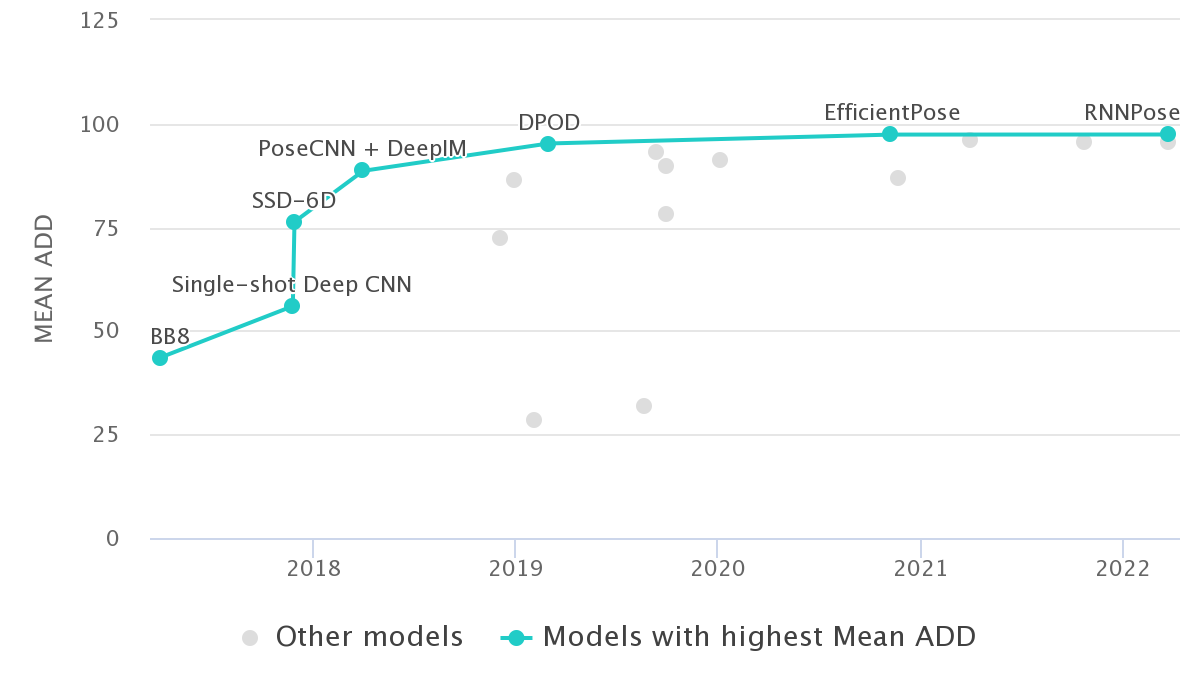
\includegraphics[width=0.7\textwidth]{linemodchart.png}
    \caption{Performance on LINEMOD of recent pose estimation algorithms by year. Graphic originates from paperswithcode.com/sota/6d-pose-estimation-on-linemod.}
    \label{fig:linemodchart}
\end{figure}

\subsection{Conclusions on Learning Approaches}

Data-driven models based on deep learning are generally considered superior to non-learning-based models. A wide variety of approaches exists, and each approach brings its own distinct advantages. When choosing a model, special attention must be given to the requirements for the application the model is destined for. Overall, recent approaches have been dominated by variations on 2D-3D correspondence and refinement methods, with a few exceptions.

\section{EfficientPose}

EfficientPose was chosen as the starting point for this thesis as it boasts state-of-the-art results while maintaining relative simplicity and low computational cost. It was designed with multi-object estimation in mind, which is especially significant, as other approaches do not scale well with the number of total detections.

Similarly to Deep-6DPose (previously mentioned in section \ref*{ss:directestimation}), it is an end-to-end direct 6D pose estimation approach that extends the functionality of a 2D network. While Deep-6D extends the segmentation network Mask-R-CNN, EfficientPose extends Google's object classification network EfficientDet\cite{EfficientDet}, which in turn builds on Google's backbone network EfficientNet\cite{EfficientNet}. We will briefly examine these two network families.

We specify "families," as both networks are based on the concept of scalability. They provide a baseline network, and then scale up its depth, width and resolution using a single hyperparameter ($\phi$) to achieve better performance when necessary. EfficientNet is designed using neural architecture search\cite{NAS} to provide optimal structure for the baseline, while EfficientDet expands upon this backbone by introducing a feature pyramid network\cite{FPN} (FPN).

FPNs are built for multi scale feature fusion, combining information contained in low resolution, semantically strong features with information containted in high resolution, semantically weak features. EfficientDet implements its own version of FPN, called bi-directional FPN, where top-down and bottom-up aggregation paths are then repeated a number of times dependant on the chosen $\phi$. The outputs of the Bi-FPN are then fed into two fully connected networks that perform class and bounding box prediction.

\begin{figure}[h]
    \centering
    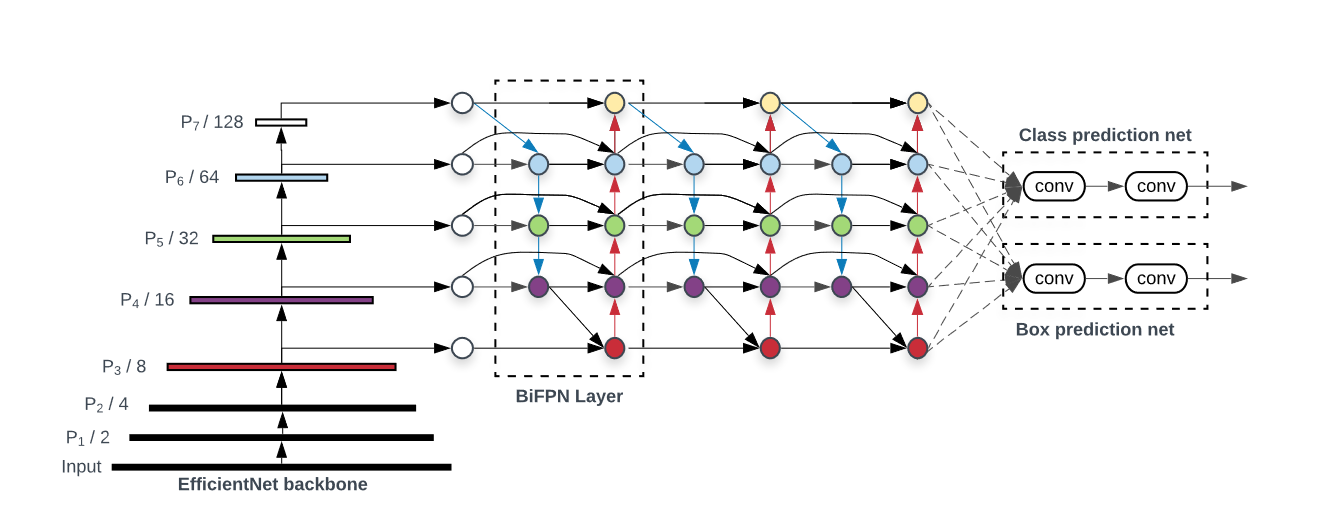
\includegraphics[width=0.9\textwidth]{EfficientDetArchitecture.png}
    \caption{Overview of the EfficientDet architecture. BiFPN layers and Class/Box layers may be repeated multiple times according to resource constraints.}
\end{figure}

\begin{figure}[ht]
    \centering
    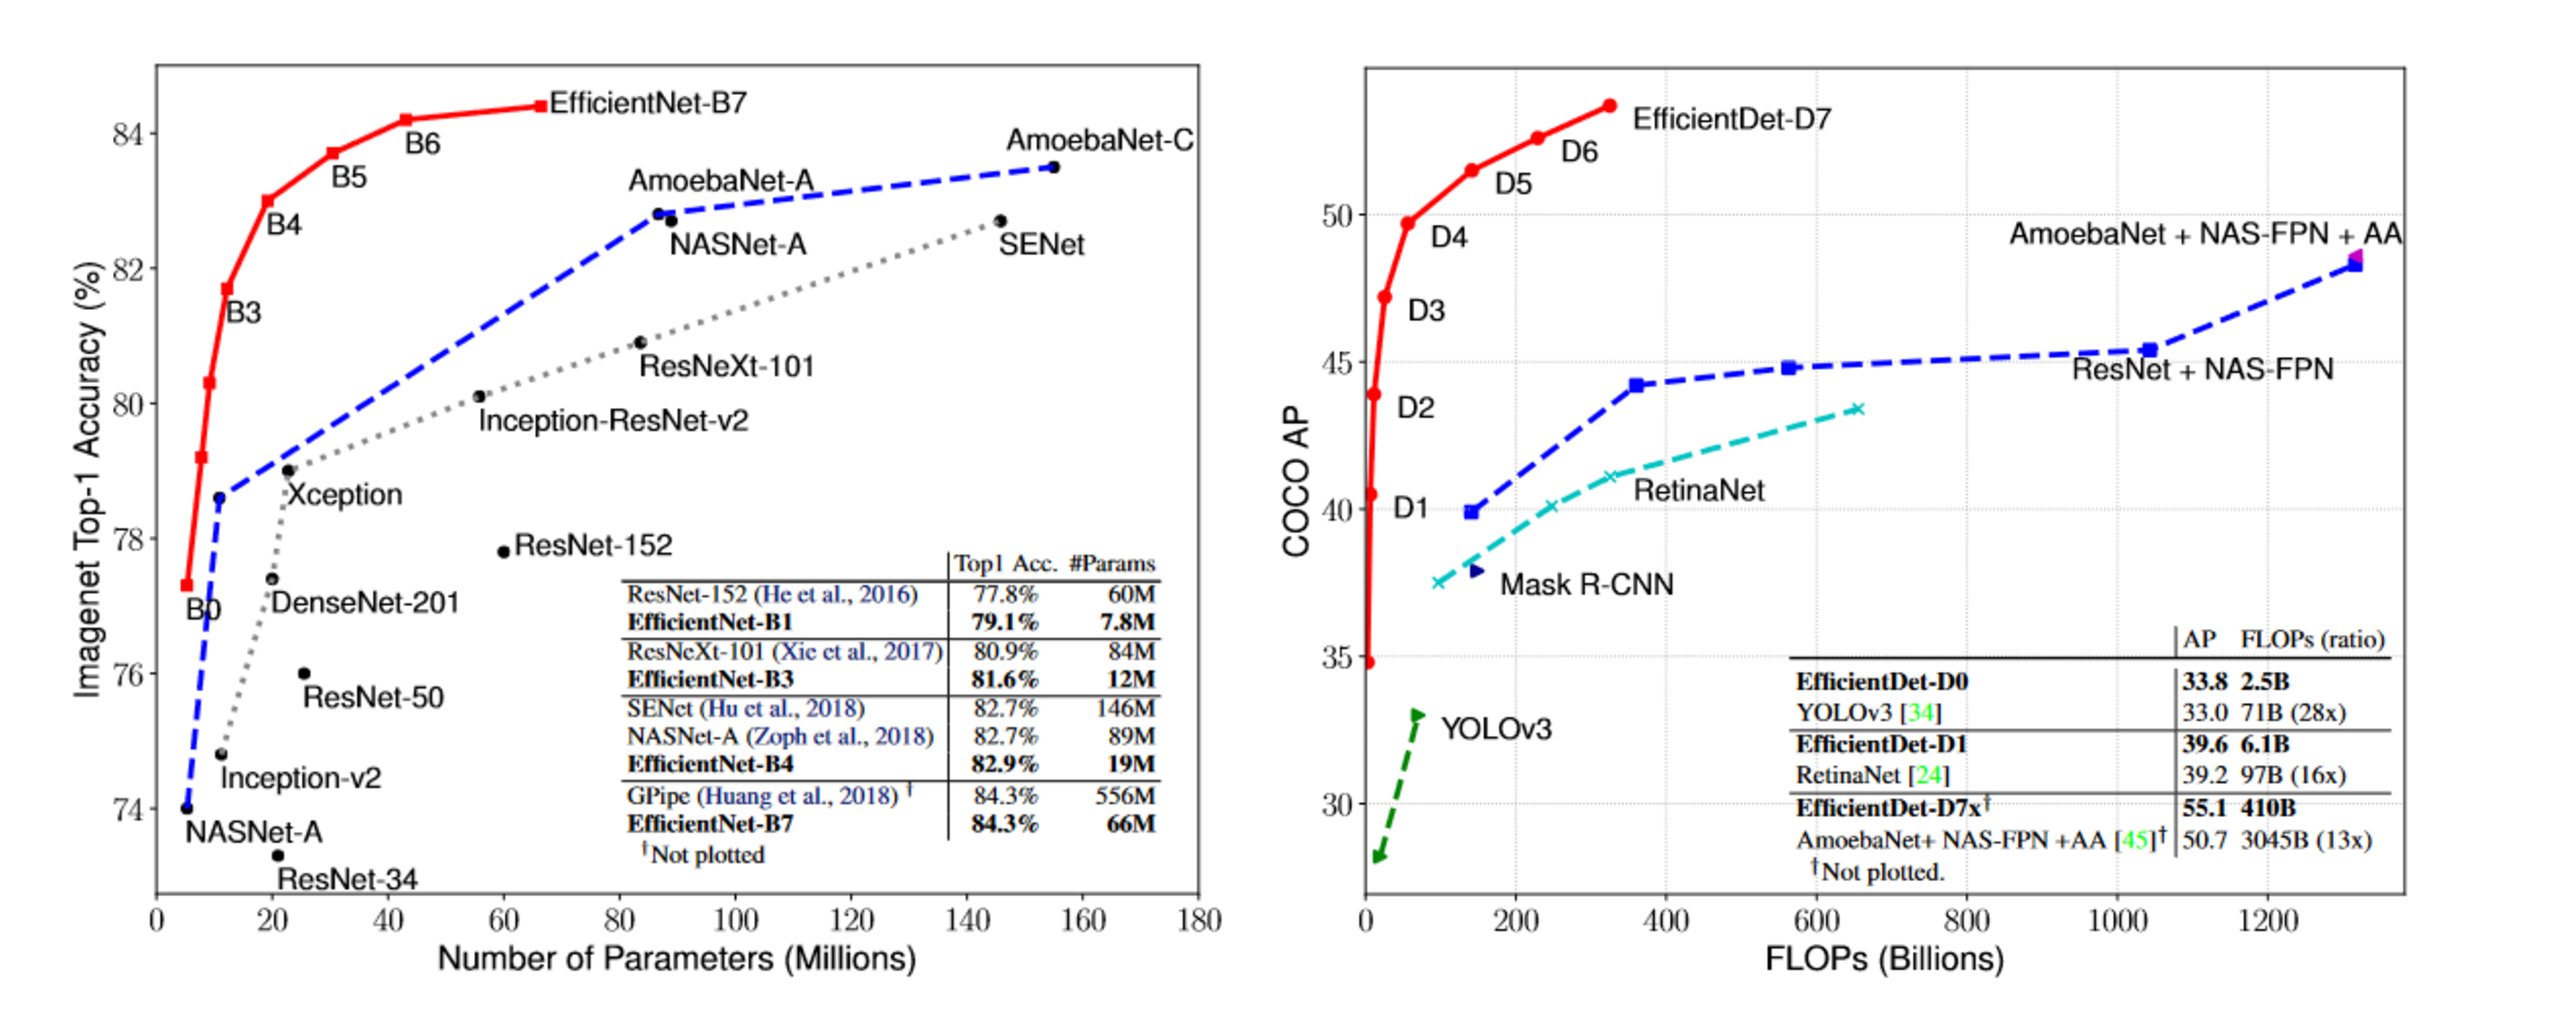
\includegraphics[width=\textwidth]{EfficientDetNetPerfromance.png}
    \caption{Performance of EfficientNet and EfficientDet relative to other approaches for various values of $\phi$. EffcientNet is evaluated on the ImageNet database\cite{imagenet}, while EfficientDet is evaluated on the Microsoft Common Objects in Context database\cite{cocodataset}. Images are taken from the relative papers on EfficientNet and EfficientDet.}
\end{figure}

The resulting network has the characteristic of being a single-shot object detector. This sets it apart from previously mentioned approaches such as Mask-R-CNN, which employ a two phase approach, with an initial region proposal step followed by the final object detection. By applying a single step approach, EfficientDet is much simpler and computationally efficient.



EfficientPose's expansion on this architecture is extremely simple, adding two additional subnets that predict translation and rotation, in parallel with the class and box networks. This means that the additional computational cost is minimal. Furthermore, while many other pose estimation approaches must be trained on a single object, EfficientPose can train and identify multiple objects at the same time, by having the subnets dedicated to each class share the same backbone and feature network.

The rotation network outputs a vector $R \in \mathbb{R}^3$ containing a minimal representation of the rotation, usually in Rodrigues angles, and then employs an additional iterative refinement strategy. Both the network size and the number of iterations are controlled by the hyperparameter $\phi$.

The translation network instead splits the task of predicting the position $p=[x, y, z]^T$ of the object into separate predictions of the 2D center $c = [c_x, c_y]^T$ and of the depth $z$. Then the final position $p$ can be computed using the camera intrinsic parameters by inverting the relationship:

\begin{equation}
    \begin{bmatrix}
        c_x\\c_y\\1
    \end{bmatrix}
    = \frac{1}{z}
    \begin{bmatrix}
        f_x & 0 & p_x \\
        0 & f_y & p_y \\
        0 & 0 & 1 
    \end{bmatrix}
    \begin{bmatrix}
        x\\y\\z
    \end{bmatrix}
\end{equation}

...where $f_x, f_y$ are the focal lengths and $(p_x, p_y)$ is the principal point. Thus we obtain:

\begin{equation}
    \begin{bmatrix}
        x\\y\\z
    \end{bmatrix}
    =z
    \begin{bmatrix}
        \frac{1}{f_x} & 0 & \frac{p_x}{f_x} \\
        0 & \frac{1}{f_y} & \frac{p_y}{f_y} \\
        0 & 0 & 1 \\
    \end{bmatrix}
    \begin{bmatrix}
        c_x\\c_y\\1
    \end{bmatrix}
\end{equation}

In summary, EfficientPose is a state-of-the-art single shot 6D pose estimator which keeps the many advantages of EfficientDets, including high accuracy, scalability, and efficency, and is relatively simple to use and modify.

\chapter{Conclusions and future developments}
\label{ch:conclusions}%
A final chapter containing the main conclusions of your research/study
and possible future developments of your work have to be inserted in this chapter.

%-------------------------------------------------------------------------
%	BIBLIOGRAPHY
%-------------------------------------------------------------------------

\addtocontents{toc}{\vspace{2em}} % Add a gap in the Contents, for aesthetics
\bibliography{Thesis_bibliography} % The references information are stored in the file named "Thesis_bibliography.bib"

%-------------------------------------------------------------------------
%	APPENDICES
%-------------------------------------------------------------------------

\cleardoublepage
\addtocontents{toc}{\vspace{2em}} % Add a gap in the Contents, for aesthetics
\appendix
\chapter*{Appendices}
\section*{Appendix A}
If you need to include an appendix to support the research in your thesis, you can place it at the end of the manuscript.
An appendix contains supplementary material (figures, tables, data, codes, mathematical proofs, surveys, \dots)
which supplement the main results contained in the previous chapters.

\section*{Appendix B}
It may be necessary to include another appendix to better organize the presentation of supplementary material.


% LIST OF FIGURES
\listoffigures

% LIST OF TABLES
\listoftables

% LIST OF SYMBOLS
% Write out the List of Symbols in this page
\chapter*{List of Symbols} % You have to include a chapter for your list of symbols (
\begin{table}[H]
    \centering
    \begin{tabular}{lll}
        \textbf{Variable} & \textbf{Description} & \textbf{SI unit} \\\hline\\[-9px]
        $\bm{u}$ & solid displacement & m \\[2px]
        $\bm{u}_f$ & fluid displacement & m \\[2px]
    \end{tabular}
\end{table}

% ACKNOWLEDGEMENTS
\chapter*{Acknowledgements}
Here you might want to acknowledge someone.

\cleardoublepage

\end{document}
